\section{Results}
\label{sec:results}

The data-driven probabilistic model we have presented produces good-looking patterns and can be applied in many different ways. The factor graph representation makes it easy to adapt our framework to handle new problems or incorporate user-provided design constraints by introducing additional factors to the factor graph, or changing the source data used to train the factor weights and histograms.

\remark{Discuss parameters used to train model ``unless otherwise specified''. Number of artists, weights, etc.}

\remark{Describe how we use the Colourlovers site to render the final images.}

\subsection{Coloring Pattern Templates}

\paragraph{Automatic pattern coloring} In the most direct application of our framework, we can sample from our model to produce colorings for a pattern template that are similar to the colorings used for training. Figure~\ref{fig:teaser} shows two examples of this process. The sampled patterns exhibit a range of colors and styles employed by the Colourlover artists. For comparison, the same patterns colored with palettes randomly sampled from RGB-space are shown on the right. These patterns exhibit significant problems, such as low color harmony and adjacent regions with equi-limuinant colors.

\begin{figure*}[ht]
\begin{tabular}{ccc}

\includegraphics[width=.15\linewidth]{figs/permutationTemplatePalette} & 
\includegraphics[width=.4\linewidth]{figs/permutationBest8} & 
\includegraphics[width=.4\linewidth]{figs/permutationWorst8} %& 
\includegraphics[width=.12\linewidth]{figs/permutationArtist}
  \\
\textbf{(a)} Input Pattern & \textbf{(b)} Highest-scoring assignments & \textbf{(c)} Lowest-scoring assignments %& \textbf{(d)} Artist assignment
\\
\end{tabular}

\caption{Given a segmented image and corresponding palette as input, we use our color model to compute the likelihood of each possible assignment of the palette to the image regions. \textbf{(b)} and \textbf{(c)} show the top-eight and bottom-eight assignments. The assignment provided by the artist received the second-highest score and is highlighted in blue.}
\label{fig:permutation}
\end{figure*}

\paragraph{Coloring with fixed palettes} In some cases, an artist already knows what colors they want to use in an image. They might have found a palette they are enamored with elsewhere, or they might have a very specific theme in mind. Even with a fixed palette, there are still a range of images that can be created by mapping different colors to different regions, only some of which are desirable. To support this task, we use our model's score to rank all possible permutations of the colors. Figure~\ref{fig:permutation} shows one example of this process. \ref{fig:permutation}b shows the eight highest-rated color assignments which exhibit a variety of color styles, such as using four different background colors. On the other hand, the lowest-rated assignments all use the tangerine background color. Our color model assigns a very low score to using this color for the background region because its color properties are not similar to background colors in the training set. The actual color assignment originally provided by the artist for this color template received the second-highest score, suggesting that our model was able to capture the artist's intent.

\begin{figure*}[ht]
\begin{tabular}{cc} 
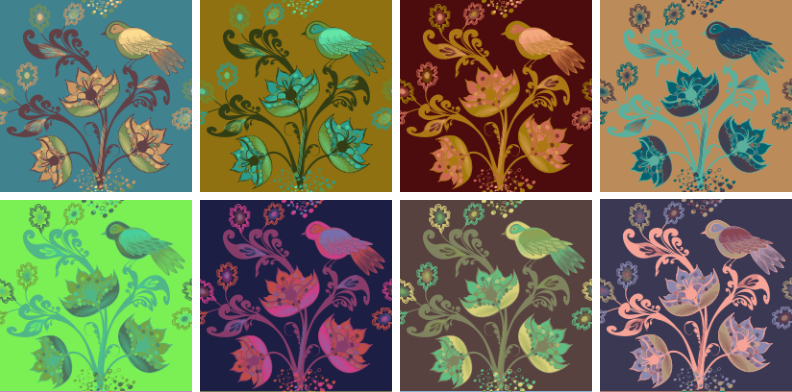
\includegraphics[width=.475\linewidth]{figs/constrainedSearchUnconstrained}&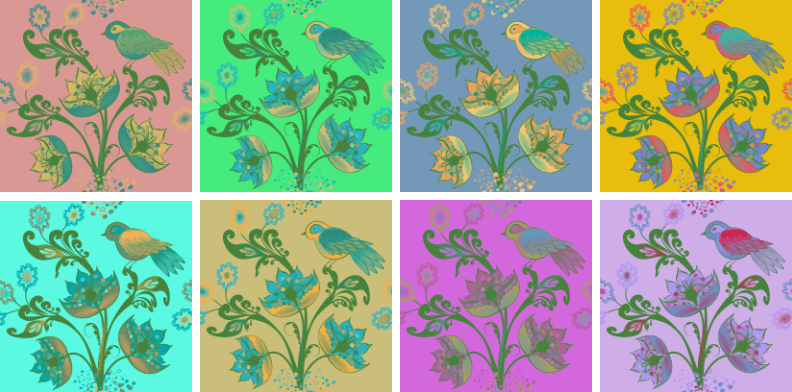
\includegraphics[width=.475\linewidth]{figs/constrainedSearchConstrained}\\
Unconstrained sampling&Constrained sampling\\
\end{tabular}

\caption{An artist coloring a pattern is presented with the results shown on the left, and decides that she only likes results where the stem of the plant is dark green. On the right, we use conditional inference to sample from our model subject to the constraint that the desired palette entry is fixed to a specific color. This is a natural way to incorporate semantic information about region colors which cannot be easily learned by our model.}
\label{fig:constrainedInference}
\vspace{-1.0em}
\end{figure*}

\remark{I realize that we may not keep in the hard or soft constraint figures and results, in favor of more ``interesting'' constraints; I'm still trying to find better examples of the hard and soft constraints though.}

\paragraph{Hard color constraints} Often a user has some idea of what types of palettes they are interested in. When this idea takes the form of a hard constraint on a region color, it is straightforward to accommodate this by using constrained inference to sample from the factor graph. Figure~\ref{fig:constrainedInference} shows an example. The model samples from the highest-scoring patterns subject to the constraint that the plant stem must be a specific shade of green.

\begin{figure}[ht]
\begin{tabular}{cc}
\raisebox{2em}{
\includegraphics[width=.22\columnwidth]{figs/guidedSearch0Original}}&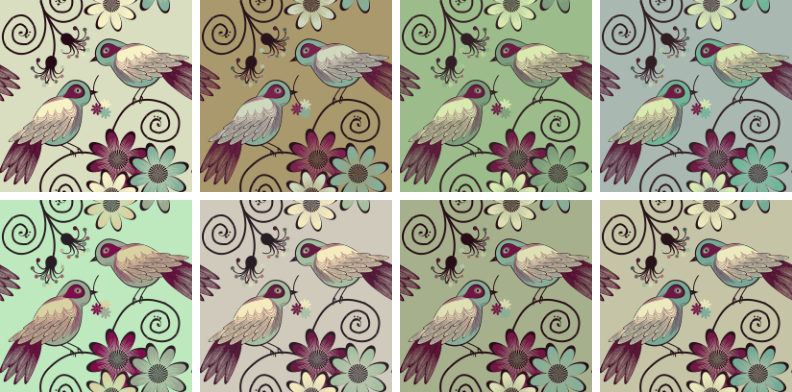
\includegraphics[width=.7\columnwidth]{figs/guidedSearch0MMR}\vspace{0.5em}\\
\raisebox{2em}{
\includegraphics[width=.22\columnwidth]{figs/guidedSearch1Original}}&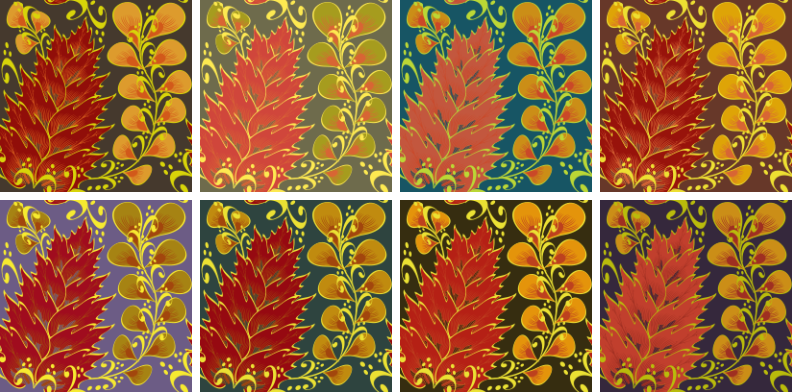
\includegraphics[width=.7\columnwidth]{figs/guidedSearch1MMR}\vspace{0.5em}\\
\raisebox{2em}{
\includegraphics[width=.22\columnwidth]{figs/guidedSearch2Original}}&
\includegraphics[width=.7\columnwidth]{figs/guidedSearch2MMR}\\
Suggestion&Results\\
\end{tabular}

\caption{An artist provides an initial color assignment and asks for patterns that are similar. We incorporate this request by adding an additional factor to our model, showing eight samples drawn from the new model for each of the suggested images.~\remark{D: It might also be cool to have a version of this that uses a photograph as the target...}}
\label{fig:nearbySuggestions}
\vspace{-1.0em}
\end{figure}

\paragraph{Soft color constraints} When the user has only a general idea of what kind of palette they want, soft constraints can be incorporated by adding new factors. A simple constraint is that the color assigned to a region should be close to a target color, which we represent using a factor of the form:

\remark{Check up on factor notation. Adds two parameters: one sigma (how far out should you search?) and one weight (what is the tradeoff between pattern-goodness and adhering to the provided colors?). May be hard to concisely summarize all this though.}

Figure~\ref{fig:nearbySuggestions} shows examples where a proposed coloring is given, and the artist asks for colorings that are similar; this results in a new factor being added to each input color region. \remark{Discussion on hold since the results will likely change}

\begin{figure}[ht]
\begin{tabular}{ccc} 
Style&Example&Results\\ %\hline
\raisebox{1.55em}{\emph{Light}}&
\includegraphics[width=.148\columnwidth]{figs/styleResultsLightExample}&
\includegraphics[width=.62\columnwidth]{figs/styleResultsLight}\vspace{0.5em}\\
\raisebox{1.55em}{\emph{Dark}}&
\includegraphics[width=.148\columnwidth]{figs/styleResultsDarkExample}&
\includegraphics[width=.62\columnwidth]{figs/styleResultsDark}\vspace{0.5em}\\
\raisebox{1.55em}{\emph{Bold}}&
\includegraphics[width=.148\columnwidth]{figs/styleResultsBoldExample}&
\includegraphics[width=.62\columnwidth]{figs/styleResultsBold}\vspace{0.5em}\\
\raisebox{1.55em}{\emph{Mellow}}&
\includegraphics[width=.148\columnwidth]{figs/styleResultsMellowExample}&
\includegraphics[width=.62\columnwidth]{figs/styleResultsMellow}\vspace{0.5em}\\
\end{tabular}

\caption{In this example, 17 patterns were chosen in three different styles, and a representative image from each style is shown in the second column. A separate model was then trained on each style, and in the third column we show four samples drawn from each model. In each case, our model is able to learn different properties of the desired distribution over colors.}
\label{fig:styleTraining}
\vspace{-1.0em}
\end{figure}

\begin{figure*}[ht]
\begin{tabular}{cc} 

\includegraphics[width=.48\linewidth]{figs/styleSugarExamples}&
\includegraphics[width=.48\linewidth]{figs/styleAlbenajExamples}\vspace{1.0em}\\
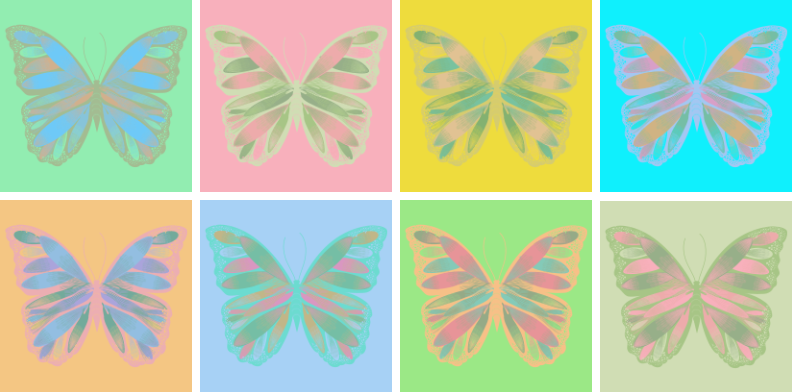
\includegraphics[width=.48\linewidth]{figs/styleSugar}&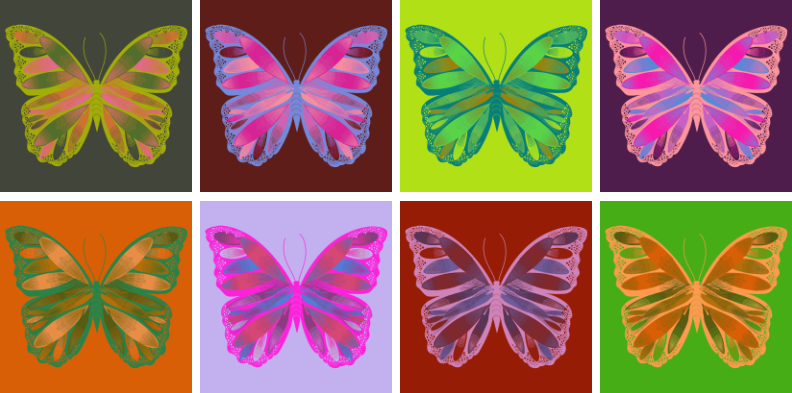
\includegraphics[width=.48\linewidth]{figs/styleAlbenaj}\\
Artist A&Artist B\\
\end{tabular}

\caption{Our data-driven approach makes it easy to capture the styles of different artists. Top: representative images from two different artists. Bottom: results sampled from a model trained on 100 images from the artist.}
\vspace{-1.0em}
\label{fig:artistTraining}
\end{figure*}

\paragraph{Style capture} A powerful advantage of a data-driven approach is the ability to modify the underlying training source to achieve specialization of the resulting model. This allows us to capture a specific style and color preferences such as ``high-contrast palettes'' simply by selecting a set of images with the desired property. Figure~\ref{fig:styleTraining} demonstrates this using four style categories: \emph{Light}, \emph{Dark}, \emph{Bold}, and \emph{Mellow}. With only 17 training examples, our model is still able to capture general properties of the images such as the distribution of colors over the background regions in \emph{Light} and \emph{Dark}, and the amount of contrast between adjacent regions in \emph{Bold} and \emph{Mellow}. It is also easy to capture the style of a specific artist, as shown in Figure~\ref{fig:artistTraining}. Here, 100 images from each artist were used for training. The sampled images mimic certain properties of the the style of each artist, such as the light backgrounds preferred by artist A and the bold colors and dark backgrounds preferred by artist B.

\subsection{Applications}

\paragraph{Web desigm}

\paragraph{3D scene design}

\subsection{Performance}

Performance figures? (training time, inference time, etc.)